\section{Evaluierung und Optimierung}

% sources:
% 1)    http://www.bioinfopublication.org/files/articles/2_1_1_JMLT.pdf

\fbox{\parbox{\textwidth}{
\noindent\textbf{Inhalt}
\begin{itemize}
    \item Theroetische Grundlagen (Confusion Matrix, ROC,  F1-Score... )
    \item Vergleich Features, ROC-Graphen, F1 Score, Confusion
    \item Bewertung
\end{itemize}
}}

Bei uns geht es um Unterscheidung von zwei Klassen, sogenanntes \emph{dichotomous binary classification problem}.

Grundlage für Analysen ist in diesem Fall die \emph{contingency table} in der \emph{true positives (tp)}, \emph{false positives (fp)}, \emph{true negatives (tn)} und \emph{false negatives (fn)} aufgetragen sind.

TODO: Table 1 aus source1

\paragraph{Precision und Recall}

\paragraph{Sensitivity und Specifity}

\paragraph{F1-Score}

Vorteile: Einfach zu berechnen und zu erklären (z.B. in Präsentationen). Bias ist einstellbar.
Nachteil: Bias

\paragraph{ROC}

Problem: Bisherige Metriken sind biased (können aber trotzdem nützlich sein). Man kann daher auch die ROC-Kurve verwenden, bei der man die Qualität des Klassifizierers (TODO Klassifikators?) ohne Bias analysieren kann.

Will man eine Zahl, kann man z.B. die Fläche unter der Kurve berechnen, es gibt aber auch andere Maße (siehe source1).

\paragraph{Beste Sachen}

Problem: ROC ist langsam.
Daher folgende Werte verwenden:
Informedness, Markedness and Matthews Correlation

Informedness und Markedness sind nützlich (TODO warum).
Matthews Correlation ist ein guter Weg beide in eine Zahl zu bekommen (ist einfach das geometrische Mittel).


\begin{figure}[!h]
    \centering
    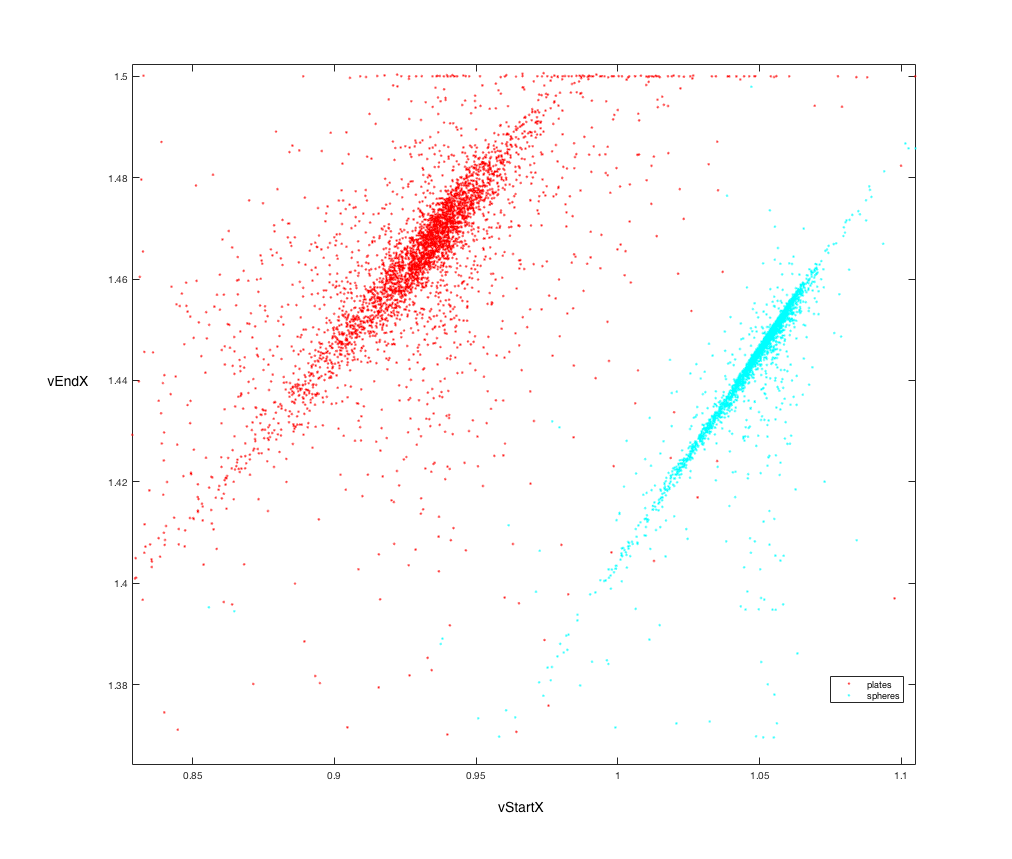
\includegraphics[width=0.7\textwidth]{pics/plotPlates-Spheres.png}
    \caption{plot Plates-Spheres}
    \label{fig:plotPlates-Spheres}
\end{figure}